\documentclass[11pt]{article}

\usepackage{layout}
\usepackage[a4paper, margin=1in]{geometry}
\usepackage{fancyhdr}
\usepackage{amsmath}
\usepackage{amsfonts}
\usepackage{amssymb}

\usepackage[utf8]{inputenc}
\usepackage{algorithm}
\usepackage{algpseudocode}
\usepackage{graphicx}
\usepackage[export]{adjustbox}
\usepackage{titlesec}
\usepackage{setspace}
\usepackage[usenames,dvipsnames]{xcolor}

\pagestyle{fancy}
\lhead{Corinna Lin | 01/28/2023}
\chead{Assignment 1}
\rhead{\thepage}
\setlength{\parindent}{0pt}

\begin{document}

\section*{Analysis:}

Highlighting Scheme:
\begin{itemize}
    \item entities will be highlighted in \colorbox{Lavender}{pink}
    \item attributes will be highlighted in \colorbox{SpringGreen}{lime}
    \item relationships will be written in \textcolor{CornflowerBlue}{blue} 
    \item constraints will be highlighted in \colorbox{pink}{peach}
    \item irrelevant information will be \textcolor{lightgray}{lightened}
\end{itemize}

\textcolor{lightgray}{A local community group is brainstorming with local artists to support artistry and share artwork with the community in a novel way via an art library that enables the local community to learn about the artists, borrow their art, and support their art (as part of the library subscription fees will return to the artists). The main component of the art library will be the art catalogue that maintains information on the art pieces that can be borrowed from the library.In addition, the art catalogue information will be used to promote art pieces and artists via the library website.} \\

\textcolor{lightgray}{Central to the art catalogue are} \colorbox{Lavender}{art pieces.}\footnote{art piece is an entity} \textcolor{CornflowerBlue}{Each} art piece has a \colorbox{pink}{unique} \colorbox{SpringGreen}{main artist} and \colorbox{SpringGreen}{title}\footnote{potentially a combined key?} \textcolor{lightgray}{(hence, two distinct artists can both make distinct art pieces named “tomorrow”). Besides the main artist,} multiple other artists can contribute to the art piece. In that case, a \colorbox{pink}{strict order of the individual contributions needs to be maintained}\footnote{potential list structure of artists? kinda a constraint but not really} \textcolor{lightgray}{(e.g., main artist, second contributor, third contributor, and so on). Typically,} art pieces also have a \colorbox{SpringGreen}{time} and \colorbox{SpringGreen}{place of creation} \textcolor{lightgray}{(for now, the library expects to only hold newly created pieces for which these details are always available). For display purposes, the} art library will maintain the \colorbox{SpringGreen}{physical dimensions} \textcolor{lightgray}{(e.g., size of a painting)} of each art piece. \\

\textcolor{lightgray}{For some types of art pieces, other details are maintained. Initially, the library will be working with talented painters, sculptors, and photographers.} For both \colorbox{Lavender}{\textcolor{CornflowerBlue}{paintings}} and \colorbox{Lavender}{\textcolor{CornflowerBlue}{photo prints}}\footnote{paintings and photo prints have potential for an ISA art piece relationship}, the library will catalogue the \colorbox{SpringGreen}{category} \textcolor{lightgray}{(e.g., still life, portrait, landscape, and so on) and the} \colorbox{SpringGreen}{coloring} \textcolor{lightgray}{(e.g., natural colors or a black-and-white color tone), and the} \colorbox{SpringGreen}{type of support material} \textcolor{lightgray}{(e.g., canvas or wood) on which the painting was made or photo was printed.} For paintings, \textcolor{lightgray}{the library will in addition} catalogue the \colorbox{SpringGreen}{type of paint used} \textcolor{lightgray}{(e.g., oil-based or water-based).} For \colorbox{Lavender}{\textcolor{CornflowerBlue}{sculptures}}\footnote{ISA relationship again}, \textcolor{lightgray}{the library will catalogue its} \colorbox{SpringGreen}{weight}\textcolor{lightgray}{, whether it can be} \colorbox{SpringGreen}{displayed indoor or outdoor} \footnote{can be stored in a boolean value}\textcolor{lightgray}{, and the} \colorbox{SpringGreen}{main material used}\textcolor{lightgray}{. Finally,} each photo print will be related to \colorbox{SpringGreen}{details} on the original photo the print was based on \textcolor{lightgray}{(e.g., the art piece is a reprint on canvas made in 2022 by Freda, based on a photo made by the photographer Xanthe in 1983). In the catalogue,} photos \textcolor{lightgray}{(the original negatives or the original digital photo file)} are \colorbox{Lavender}{non-physical} \footnote{maybe separate physical and non-physical pieces into entities?} art pieces: they \colorbox{pink}{cannot be borrowed} from the library and \colorbox{pink}{do not have physical dimensions}, but do have titles, an artist that created them, other contributors, and a time and place of creation. \\

For \textcolor{CornflowerBlue}{each} \colorbox{Lavender}{artist}\textcolor{lightgray}{, the library maintains a} \colorbox{Lavender}{profile page} \footnote{will connect the artist entity to their art pieces (entities)} \textcolor{lightgray}{that is used to highlight the artist and via which} \colorbox{pink}{one can find all art pieces of that artist in the catalogue}. \textcolor{CornflowerBlue}{Each} artist profile displays their \colorbox{SpringGreen}{name}, their \colorbox{SpringGreen}{current location} \textcolor{lightgray}{(e.g., Hamilton if that is the location of their main atelier), and their} \colorbox{SpringGreen}{age}. \textcolor{lightgray}{In addition,} the artist can
add links to \colorbox{Lavender}{external resources}\footnote{must be an entity because attributes cannot have complex data structures} \textcolor{lightgray}{such as personal websites, Instagram pages, YouTube channels, and so on.} \\

Art pieces can be \textcolor{CornflowerBlue}{grouped} together\textcolor{lightgray}{, e.g., they can be part of the same collection(s), or they can be part of a group of art pieces made within a collaboration.} \textcolor{CornflowerBlue}{Each} such a group has a \colorbox{SpringGreen}{title}, \colorbox{SpringGreen}{type}, and \colorbox{SpringGreen}{description}\textcolor{lightgray}{. Several groups can have the same title, types, and/or descriptions.} \\

\textcolor{lightgray}{Finally, the library will have} \colorbox{Lavender}{members} that \textcolor{CornflowerBlue}{can borrow} art pieces. \textcolor{lightgray}{The library plans to a pre-existing system to manage memberships and payment details. This system will} assign a \colorbox{pink}{unique} \colorbox{SpringGreen}{member id} \colorbox{pink}{to each member}\textcolor{lightgray}{. That system will not manage the borrowed and reserved art pieces, however.} \textcolor{CornflowerBlue}{Each borrowed work is associated with an art piece, the member that borrowed it, and the} \colorbox{SpringGreen}{\textcolor{CornflowerBlue}{time period}} during which the work is borrowed. \textcolor{CornflowerBlue}{Each reserved work is associated with an art piece, the member that wants to borrow it, and the time when the reservation was placed} \colorbox{pink}{(reserving art pieces works on a first-come first-serve basis)}. Members can \colorbox{pink}{borrow the same art piece multiple times} and members can \colorbox{pink}{indefinitely renew their borrow} \colorbox{pink}{period unless other members have reserved the piece} (each renew is registered as a separate borrow).

\newpage

\section*{Solution:}

For this assignment, I have derived an ER-Diagram that represents all information (hopefully) present in the description provided. The ER-Diagram can be found in Figure 1. The following is a high-level overview of my ER-Diagram where I will discuss the choices I made and present any constraints. I will go sequentially, according to the description. \\

The description describes that art would be shared through an art library that contains an art catalogue. Though these are nouns and may be shown in ER-Diagrams as entities, I decided that my diagram as a whole would represent the system that the art library and art catalogue would use. As such, art library and art catalogue are not represented by entities, but rather the diagram as a whole. \\

Art pieces are represented using the weak entity \textbf{Art Piece}, which are owned by the main artist, where artists as a whole are represented using the entity \textbf{Artist}. Art pieces are created by an artist, so they should be owned by the artist because the art would not exist without the artist. This is why I chose to make \textbf{Art Piece} a weak entity. Within the description, each art piece had a main artist, but could also have many other artists that contributed. Though main artist and sub-artists can be shown using an ISA hierarchy branching from \textbf{Artist} (since they are artists), it would be difficult to use the main artist as an identifier for each art piece as the description mentioned. Having said this, I decided to create two relationships between \textbf{Art Piece} and \textbf{Artist}, \textit{Main\_Artist} and \textit{Sub-Artist}. \textbf{Art Piece} is a weak entity that must participate in its identifying relationship \textit{Main\_Artist} exactly once. \textit{Sub-Artist} is a many-to-many relationship because many artists can be a sub-artist of an art piece, and multiple art pieces can have an artist as their sub-artist. In order to keep a strict order of contributions, \textit{Sub-Artist} also has an attribute \textcolor{CornflowerBlue}{order} (of type INTEGER) that will store the rank of the artist's contribution. Along with this, \textbf{Art Piece} has a partial key \textcolor{CornflowerBlue}{title} (of type TEXT) that represents the title of the art piece. Names can change and may not be unique, as such, each \textbf{Artist} will have a numeric automatically generated identifier \textcolor{CornflowerBlue}{aid} (of type INTEGER). Now, each \textbf{Art Piece} will have a main artist and a title. Since they are keys and partial keys, it can be identified through its unique combination of \textcolor{CornflowerBlue}{title} and \textcolor{CornflowerBlue}{aid}. Each \textbf{Art Piece} will also have the attributes \textcolor{CornflowerBlue}{time} (of type TIME) and \textcolor{CornflowerBlue}{place\_of\_creation} (of type TEXT), as the description describes. \\

There are 4 types of art pieces: paintings, photo prints, sculptures, and photos. With the exception of photos, all the art pieces can be borrowed or reserved. Having said this, I decided to divide the art pieces into physical and non-physical pieces, shown by the entities \textbf{Physical} and \textbf{Non-Physical}. They are still art pieces because they participate in an ISA relationship with \textbf{Art Piece}. From there, physical art pieces will have physical dimensions, which is why \textbf{Physical} has the attributes \textcolor{CornflowerBlue}{length} (of type INTEGER), \textcolor{CornflowerBlue}{width} (of type INTEGER), and \textcolor{CornflowerBlue}{height} (of type INTEGER). Paintings are represented using the entity \textbf{Painting} and as the description provides, has the attributes \textcolor{CornflowerBlue}{category} (of type TEXT), \textcolor{CornflowerBlue}{coloring} (of type TEXT), \textcolor{CornflowerBlue}{support\_material} (of type TEXT), and \textcolor{CornflowerBlue}{paint\_type} (of type TEXT). Photo prints are represented using the entity \textbf{Photo\_Print} and as the description provides, have the attributes \textcolor{CornflowerBlue}{details} (of type TEXT), \textcolor{CornflowerBlue}{category} (of type TEXT), \textcolor{CornflowerBlue}{coloring} (of type TEXT), and \textcolor{CornflowerBlue}{support\_material} (of type TEXT). Sculptures are represented by the entity \textbf{Sculpture} and as the description provides, have the attributes \textcolor{CornflowerBlue}{main material} (of type TEXT), \textcolor{CornflowerBlue}{weight} (of type INTEGER) (in this case, the weight will be rounded to a whole number and will be measured in kg), and \textcolor{CornflowerBlue}{indoor display} (of type BOOLEAN) which will be true if it can be displayed indoors and false if it cannot. All 3 types of art pieces participate in an ISA relationship with \textbf{Physical} and as such are also an \textbf{Art\_Piece}. Photo's are represented by the entity \textbf{Photo} and participate in an ISA relationship with \textbf{Non\_Physical} and are therefore also an \textbf{Art\_Piece} so it will inherit its attributes, like the other physical art pieces. \\

Each artist also has a profile page that is represented by the weak entity \textbf{Profile\_Page}. It is a weak identity because the page is owned by an artist. Without the artist, there would be no profile page because the artist does not exist. \textbf{Profile\_Page} must participate in its identifying relationship \textit{Has\_A} exactly once. \textbf{Artist} must also participate in this relationship exactly once because an artist must have a profile page and a profile page must be owned by one \textbf{Artist}. As the description describes \textbf{Profile\_Page} has the attributes \textcolor{CornflowerBlue}{current\_location} (of type TEXT), \textcolor{CornflowerBlue}{age} (of type INTEGER), and \textcolor{CornflowerBlue}{name} (of type TEXT). Along with this, since names are not unique, each profile page will also have a numeric automatically generated identifier \textcolor{CornflowerBlue}{pid} (of type INTEGER). External resources are represented using the weak entity \textbf{External\_Resources} and have the partial key \textcolor{CornflowerBlue}{url}. \textbf{External\_Resources} is a weak entity because it would not exist without a profile page. It must participate in its identifying relationship \textit{Linked\_To} which represented the external resources being linked to the profile page. A profile pages can have multiple external resources, and an external resource can be linked to multiple profile pages (for example, if it is a group of artists using a shared account). Since we are working with partial keys, even though multiple profile pages have the same url, the combination of \textcolor{CornflowerBlue}{url}, \textcolor{CornflowerBlue}{pid}, and \textcolor{CornflowerBlue}{aid} would still be unique. You must also be able to find all the artist's art pieces through their profile page. To represent this, \textbf{Profile\_Page} and \textbf{Art\_Piece} both participate in a relationship \textit{Connected\_To}. Multiple art pieces can be connected to a profile page and multiple profile pages can be connected to an art piece (through sub-artists). As such, \textit{Connected\_To} is a many-to-many relationship. \\

Art pieces can be grouped together, which is represented through a self relationship \textit{Collection} that is connected to \textbf{Art\_Piece}. A self relationship was used because collections are simply a group of multiple art pieces. As the descriptio describes, \textit{Collection} has the attributes \textcolor{CornflowerBlue}{title} (of type TEXT), \textcolor{CornflowerBlue}{type} (of type TEXT), and \textcolor{CornflowerBlue}{description} (of type TEXT). \\

Members have a unique member id. As such, members are represented using the entity \textbf{Member}, with a numeric automatically generated identifier \textcolor{CornflowerBlue}{mid} (of type INTEGER). The borrowing system is represented using the \textit{Borrow} relationship that has the attribute \textcolor{CornflowerBlue}{time\_period} (of type TEXT) to describe the time period the art piece is borrowed, and \textcolor{CornflowerBlue}{reserved} (of type BOOLEAN) which will be true if the art piece is reserved and false if it is not. The entities \textbf{Member} and \textbf{Physical} participate in this relationship. \textbf{Physical} specifically has a one-to-many participation. This is because a physical art piece can only be borrowed by one member at a time, however, members can borrow multiple art pieces at once. Having said this, if the attribute \textcolor{CornflowerBlue}{reserved} is true, the member cannot re-borrow the art piece because it it reserved. If reserved is false, the member can indefinitely renew their borrowed art piece. Though the description says that members can borrow the same art piece multiple times, I interpret this as renewing the same art piece multiple times (like a chain), so the one-to-many participation remains. Reservations are represented using the \textbf{Reservation} weak entity and have the attributes \textcolor{CornflowerBlue}{time\_placed} (of type TIME), \textcolor{CornflowerBlue}{time\_period} (of type TEXT) (this was not in the description, however, it made sense to me that a member would reserve the art piece for a certain amount of time. Members also wouldn't be able to reserve an art piece for a time period that the art piece is already reserved for, but this is not described in the diagram.), and \textcolor{CornflowerBlue}{place\_in\_queue} (of type INTEGER) in order to keep the first-come first-served basis. None of these attributes can be guaranteed to be unique, so there is also a numeric automatically generated identifier (partial key) \textcolor{CornflowerBlue}{rid} (of type INTEGER). \textbf{Reservation} is a weak entity that is owned by \textbf{Member} because reservations must be made by a member, and without a member to make a reservation, reservations would not exist. \textbf{Member} and \textbf{Reservation} participate in the relationship \textit{Make\_Reservation}. This relationship represents creating a reservation for an art piece. \textbf{Reservation} must participate in this identifying relationship exactly once because a reservation must be made by a member. This is made under the assumption that only one member can own a reservation, as in multiple members cannot group and create one reservation. However, a member can make multiple reservations, which is still depicted in the relationship. Once the reservation is made, the art piece will be reserved for the \textcolor{CornflowerBlue}{time\_period}, assuming the art piece is not reserved for the time period already (which is not depicted in the diagram). This is represented through the \textit{Reserve} relationship. \textbf{Reservation} must participate in this relationship exactly once because a reservation must be related to a single art piece. Art pieces can have multiple reservations which is why there are no restrictions from \textbf{Physical} to \textit{Reserve}. Once an art piece is reserved, the \textcolor{CornflowerBlue}{reserved} attribute in the \textit{Borrow} relationship will also be true, which is also not depicted in this diagram.

\begin{center}
\begin{figure}[H]
    \caption{ER-Diagram}
    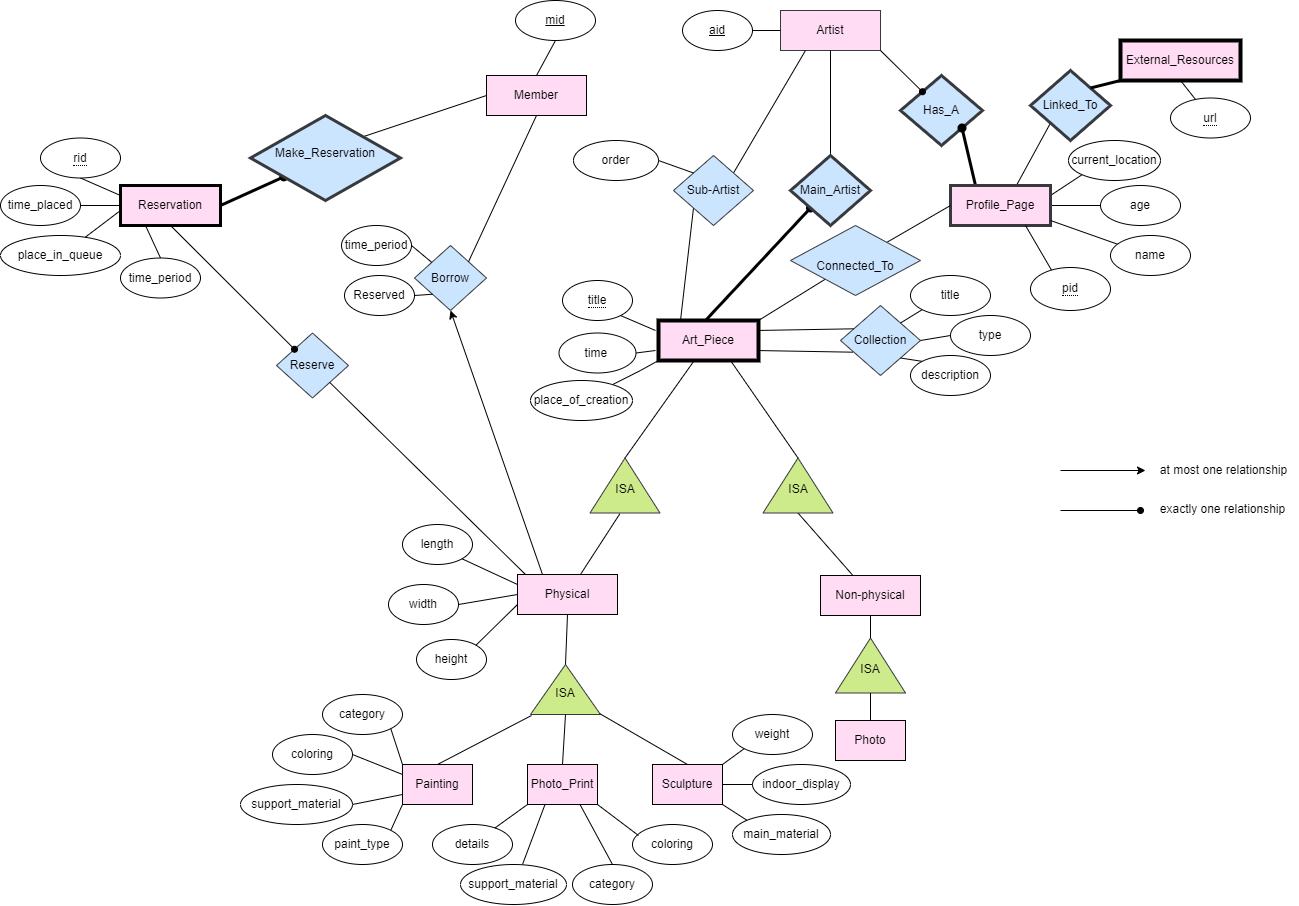
\includegraphics[width=18cm]{ER_Diagram.png}
\end{figure}
\end{center}

\end{document}